%!TEX root = ../template.tex
%%%%%%%%%%%%%%%%%%%%%%%%%%%%%%%%%%%%%%%%%%%%%%%%%%%%%%%%%%%%%%%%%%%
%% chapter1.tex
%% NOVA thesis document file
%%
%% Chapter with introduction
%%%%%%%%%%%%%%%%%%%%%%%%%%%%%%%%%%%%%%%%%%%%%%%%%%%%%%%%%%%%%%%%%%%

\typeout{NT FILE proposed_work.tex}%

\chapter{Proposed Work}
\label{cha:proposed_work}

\prependtographicspath{{Chapters/Figures/Covers/}}

% epigraph configuration
\epigraphfontsize{\small\itshape}
\setlength\epigraphwidth{12.5cm}
\setlength\epigraphrule{0pt}

This chapter outlines the expected contributions of this research, which aims to address these gaps by providing a structured approach to ethical requirements engineering.

% \section{Results from the Systematic Mapping Study}
% The results of the Systematic Mapping Study (SMS) reveal a diverse set of approaches for specifying ethical requirements in software engineering, ranging from structured methodologies like ObRE 
% and GORE to user-centered methods such as SPIDe and OpenEHR archetypes, and automated techniques like ReFAIR. While these approaches offer valuable frameworks for integrating ethics into 
% software design, they face challenges such as scalability, context dependency, and the need for specialized knowledge or stakeholder involvement. Despite these limitations, many approaches 
% demonstrate flexibility, adaptability, and a strong focus on ensuring ethical compliance, particularly in areas like fairness and user needs alignment. The study underscores the importance of 
% balancing structured processes with flexibility to address the evolving complexities of ethical requirements in real-world software development.

\section{Approach for Ethical Requirements Specification}
We aim to contribute with an approach that helps solve a present problem in Requirements Engineering for Software products.

Our intended approach for ethical requirements elicitation is a software tool that with the support of a UI is able to accept the concept for a software idea of a User, and with the help of OpenAI's chat GPT, and
the ECCOLA method, it will generate a specfication of Ethical User Stories to be implemented during the development stage. This approach is inteded to be accessible and use LLMs to simulate the discussion
between several colaborators and the User.

In the figures \ref{fig:BPMN_Tese_ver4_part1} and \ref{fig:BPMN_Tese_ver3_part2} it is represented the BPMN of the approach we intend to follow. 
It is divided in two parts for better understanding. Our tool starts with receiving the User's software idea as an input, then it uses ChatGPT to generate a set of Agents with different personalities,
these agents will discuss how the system works in order to have a full understanding of it. After that, according to the ECCOLA method \cite{VAKKURI2021111067} the agents will define a set of Sprints
required to developed the software and confirm with the User. If the User agrees, the tool will choose the ECCOLA cards that are relevant for each Sprint, discussing with each other each card's questions
as well as questioning the User. The agents will then generate Ethical requirements based on the previous discussions and the User's feedback. Finally, defining a specification of Ethical User Stories to be
implemented during the development stage.

\begin{figure}[h]
    \centering
    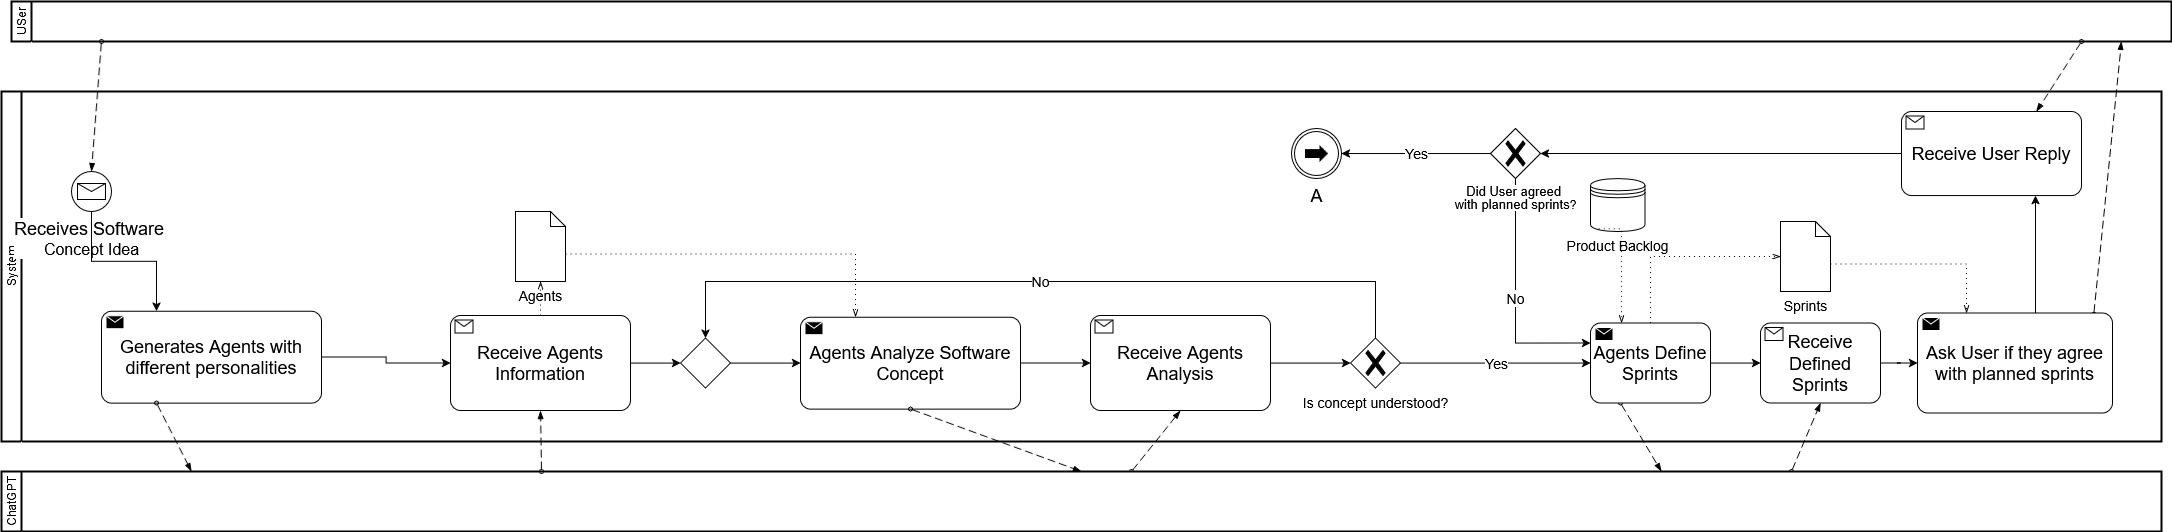
\includegraphics[width=1.1\textwidth]{BPMN_Tese_ver4_part1}
    \caption{Our approache BPMN part 1}
    \label{fig:BPMN_Tese_ver4_part1}
  \end{figure}

\begin{figure}[h]
    \centering
    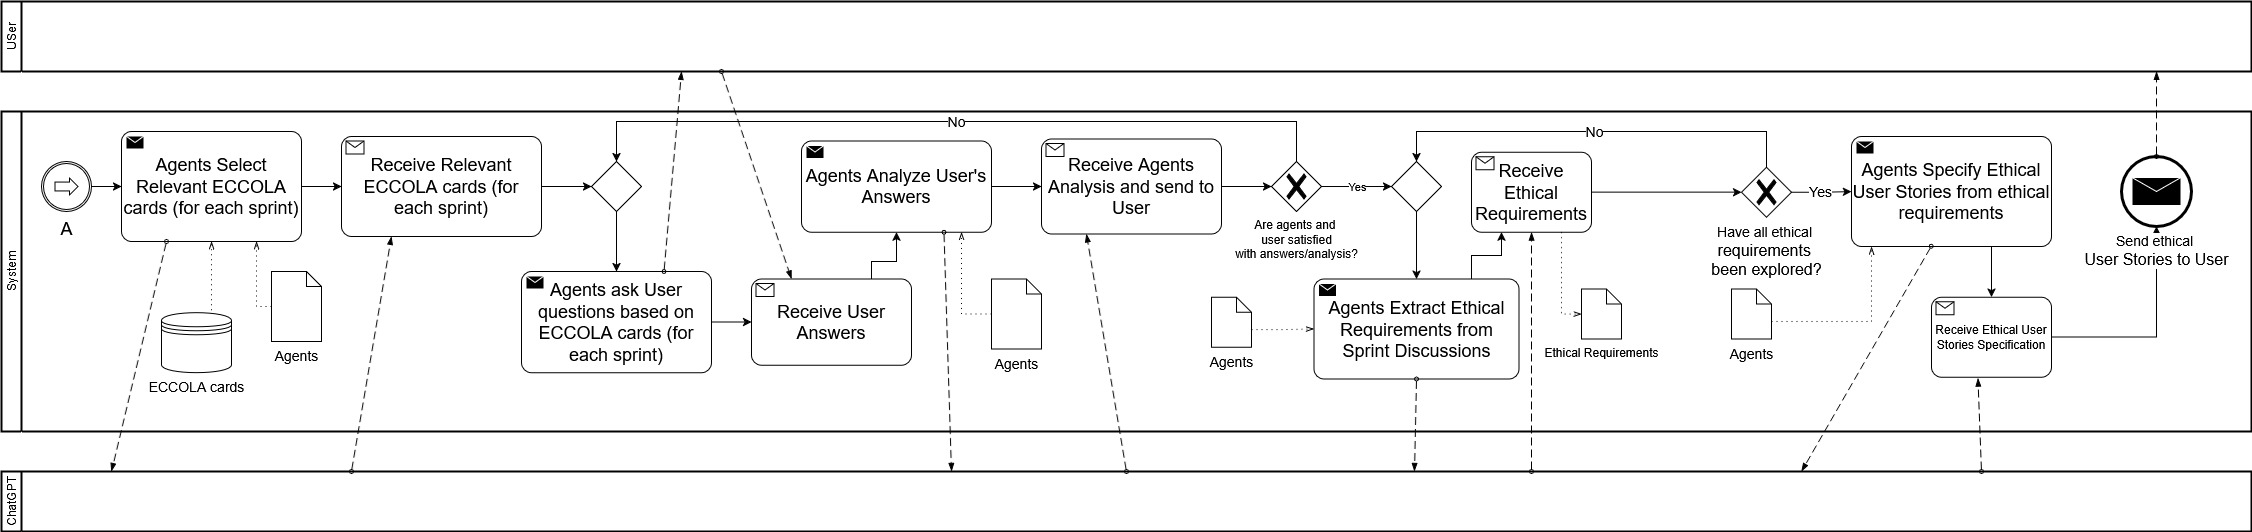
\includegraphics[width=1.1\textwidth]{BPMN_Tese_ver3_part2}
    \caption{Our approache BPMN part 2}
    \label{fig:BPMN_Tese_ver3_part2}
  \end{figure}

\subsection{User Stories Evaluation}
In this section, we discuss the metrics with which the ethical user stories generated
will be evaluated. To achieve this, we used a version of the metrics provided by Lucassen et al. \cite{b22} adapted to our use case.
To evaluate the user story quality, the authors use syntactic metrics, such as \textit{Well-formed}, \textit{Atomic}, and \textit{Minimal}, which assess the textual structure of the US, disregarding its meaning. Semantic metrics, such as \textit{Conceptually sound} and \textit{Problem-oriented}, which focus on the meaning of the US text. Pragmatic metrics, such as \textit{Unique and conflict-free}.

We propose %followed 
the following structure for our metrics:
\begin{itemize}
    \item \textbf{Well-formed}: Ethical User Stories need to have a correct format and structure by including at least an actor, an ethical concern, an ethical principle, a consequence/harm, a mitigation, and an ECCOLA card alignment. We score each element as follows:
    0 - If it isn't included, 0.5 - If it was not clear, 1 - If it's included. The total score can be a maximum of 7.
    
    \item \textbf{Atomic}: EUSs can only describe one ethical concern or issue. We score as follows:
    0 - If it isn't described, 0.5 - If it was not clear, 1 - If it's described. The total score can be a maximum of 1.

    \item \textbf{Minimal}: EUSs don't have redundant info, including only ethics-relevant elements. We score as follows:
    0 - If there are more elements, 0.5 - If it was not clear, 1 - If there are not more elements. The total score can be a maximum of 1.

    \item \textbf{Conceptually sound}: Each element of the EUS (actor, ethical principle, consequence/harm, mitigation, and ECCOLA card alignment) expresses exactly its purpose. We score each element as follows:
    0 - If it isn't expressed, 0.5 - If it was not clear, 1 - If it's expressed. The total score can be a maximum of 7.

    \item  \textbf{Problem-oriented}: The ethical mitigation of EUSs should address the specified ethical concern directly. We score as follows:
     0 — If it does not mitigate; 0.5 — If it was not clear; 1 — If it mitigates. The total score can be a maximum of 1.

     \item \textbf{Unique and conflict-free}: Each EUS should be unique, having no other EUS that is semantically equal or too similar. We score as follows:
     0 - If it is not unique, 0.5 - If it was not clear, 1 - If it is unique
\end{itemize}

With these metrics, we can analyze the quality of the EUSs generated by the personas in our system, assessing the completeness and clarity of ethical concerns and their mitigations, we can ensure the alignment with ECCOLA cards and, identify ambiguous EUS. Moreover, we should ensure the EUS alignment with the European Union guidelines for Trustworthy AI\footnote{https://ec.europa.eu/info/funding-tenders/opportunities/docs/2021-2027/horizon/guidance/ethics-by-design-and-ethics-of-use-approaches-for-artificial-intelligence\_he\_en.pdf}.

\section{Advancing Ethical Requirements Elicitation Research}
Through this study and the development of our method, we intend to further advance the research in the field of Ethical Requirements Elicitation, with our developed approach.

\section{AI in Ethical Requirements Engineering}
We aim to contribute to the field of AI in Ethical Requirements Engineering by demonstrating LLMs interpretational capabilities to assist Reqruiements Engineers in the elicitation of
Reqruiements derived from abstract, or ethical, concepts, which often require a more human oriented approach.


\section{Work Plan}
The work plan for this research is structured into several stages, as illustrated in the Gantt chart in Figure \ref{fig:gantt_chart}. The first stage involves developing 
the framework's architecture, followed by conducting experiments to test the proposed approach. Next, we proceed with the implementation phase, after which we validate our approach by comparing the 
results with previous studies and experiments, as well as evaluating it with potential users. Finally, we complete the process by writing the final thesis document.

\begin{figure}[h]
  \centering
  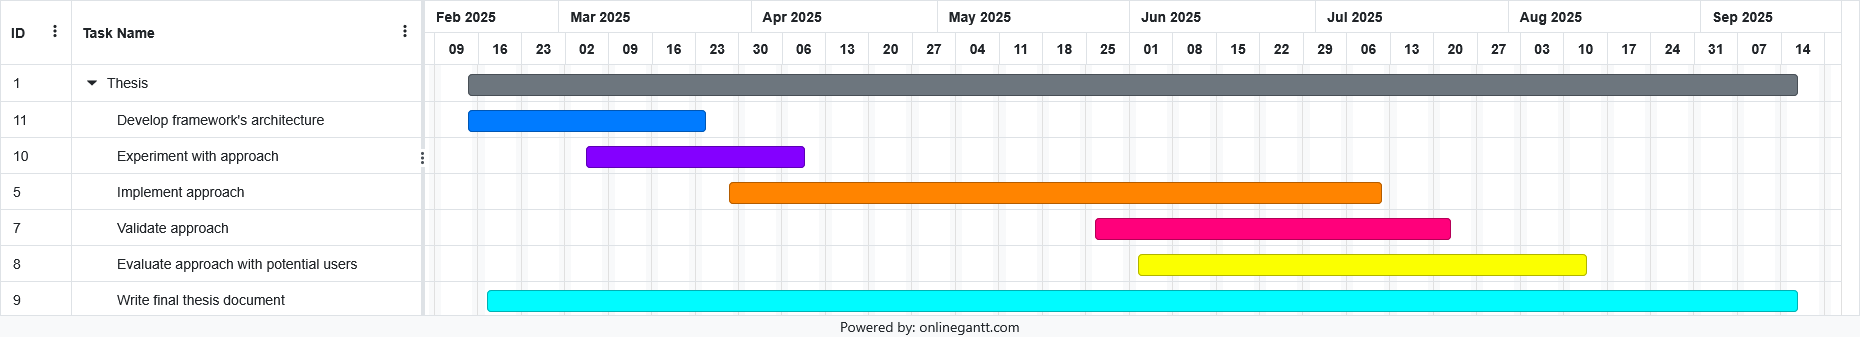
\includegraphics[width=1.1\textwidth]{gantt_chart}
  \caption{Work Plan Gantt Chart}
  \label{fig:gantt_chart}
  \end{figure}